\documentclass{primedoc}
\usepackage{amsmath}
\usepackage{amssymb}
\usepackage{tikz}
\usetikzlibrary{arrows.meta}
\usepackage{microtype}
\usepackage{booktabs}
\usepackage{minted}
\setminted{style=friendly,fontsize=\small}
\renewcommand{\listoflistingscaption}{List of Code Listings}
\usepackage{hyperref}  % for hyperlinks
\usepackage[a4paper,top=4.2cm,bottom=4.2cm,left=3.5cm,right=3.5cm]{geometry} % for setting page size and margins


\usepackage[framemethod=TikZ]{mdframed}
\newcounter{thm}[section]\setcounter{thm}{0}
\renewcommand{\thethm}{\arabic{section}.\arabic{thm}}
\newenvironment{thm}[2][]{%
\refstepcounter{thm}%
\ifstrempty{#1}%
{\mdfsetup{%
frametitle={%
\tikz[baseline=(current bounding box.east),outer sep=0pt]
\node[anchor=east,rectangle,fill=blue!20]
{\strut Theorem~\thethm};}}
}%
{\mdfsetup{%
frametitle={%
\tikz[baseline=(current bounding box.east),outer sep=0pt]
\node[anchor=east,rectangle,fill=cyan!20]
{\strut Theorem~\thethm:~#1};}}%
}%
\mdfsetup{innertopmargin=10pt,linecolor=blue!20,%
linewidth=2pt,topline=true,%
frametitleaboveskip=\dimexpr-\ht\strutbox\relax
}
\begin{mdframed}[]\relax%
\label{#2}}{\end{mdframed}}


% Custom macros used in this example document
\newcommand{\doclink}[2]{\href{#1}{#2}\footnote{\url{#1}}}
\newcommand{\cs}[1]{\texttt{\textbackslash #1}}

% Frontmatter data; appears on title page
\title{Google PageRank Algorithm}
\subtitle{An Application of Linear Algebra}
\author{Manish Patel}
\softwarelogo{
\includegraphics[width=8cm]{img}}
\begin{document}
\maketitle
\newpage
~\vfill
\thispagestyle{empty}
\noindent \copyright\ Manish Patel\\ % Copyright notice
\noindent \textsc{The Institute of Science, Mumbai}\\ % Publisher	
\noindent \textit{primespatel@gmail.com}\\ % URL	
\noindent \textit{2021-22}
\newpage
\tableofcontents
% \listoflistings%
\newpage

\section{Introduction}
Humans, the most successful species on the planet, used to pass on their knowledge through books, music, art, and so on. This knowledge transfer continues to this day, but with the most popular, innovative, and easily accessible source that is also a reliable alternative, you guessed it, the Internet. One can conduct a search. What exactly are prime numbers? Google returns n related pages, with the most relevant appearing first.\newline
	
\noindent The process of searching within a document collection for specific information is known as information retrieval (called a query).\\
\\
An information retrieval challenge for any document collection, especially the Web which concerns precision. The amount of accessible information continues to grow, a user's ability to look at documents does not. Users rarely look beyond the first 10 or 20 documents retrieved. This user impatience means that search engine precision must increase just as rapidly as the number of documents is increasing.\\
\\
The Web is such a unique document collection which is huge, dynamic, self-organized, and hyperlinked. The Web's self-organization means that, in contrast to traditional document collections, there is no central collection and categorization organization. The web document collection lives in a cyber warehouse, a virtual entity that is not limited by geographical constraints and can grow without limit.
\section{Elements of Web Search Engine}
	
\subsection{Crawler Module}
Web is huge and dynamic in nature as a result, all web search engines have a crawler module. This module contains the software that collects and categorizes the web's documents. The crawling software creates virtual robots, called spiders, that constantly crawls the Web gathering new information and webpages and returning to store them in a central repository.
	
\subsection{Page Repository}
The spiders return with new webpages, which are temporarily stored as complete webpages in the page repository. The new pages remain in the repository until they are sent to the indexing module, where their vital information is stripped to create a compressed version of the page.

\begin{figure}[h]
    \centering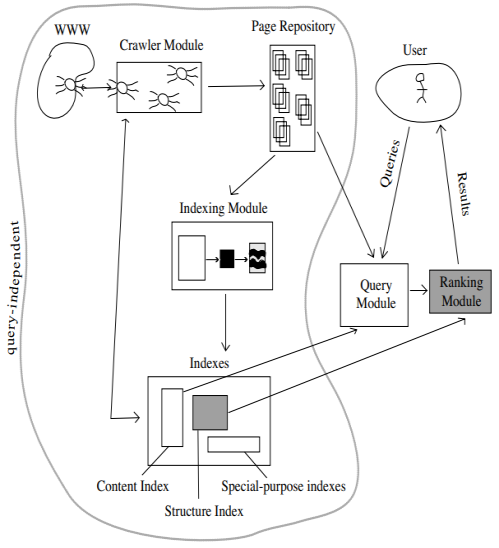
\includegraphics[scale=0.5]{engine.png}
    \caption{Elements of Web Search Engine}
    \label{fig:placeholder} % Unique label used for referencing the figure in-text
            %\addcontentsline{toc}{figure}{Figure \ref{fig:placeholder}} % Uncomment to add the figure to the table of contents
    \end{figure}

\subsection{Indexing Module}
The indexing module takes each new uncompressed page and extracts only the vital descriptors, creating a compressed description of the page that is stored in various indexes. The indexing module is like a black box function that takes the uncompressed page as input and outputs a “Cliffnotes” version of the page. The uncompressed page is then tossed out. We will be concentrating in PageRank index in this module.

\subsection{Indexes}
The indexes hold the valuable compressed information for each webpage. The first is called the content index. Here the content, such as keyword, title, and anchor text for each webpage, is stored in a compressed form using an inverted file structure. The crawler module sometimes accesses the structure index to find uncrawled pages. information regarding the hyperlink structure of pages in the search engine's index is gleaned during the indexing phase. This link information is stored in compressed form in the structure index. Special-purpose indexes are the final type of index. For example, indexes such as the image index and pdf index hold information that is useful for particular query tasks.\\
\\
The four modules above (crawler, page repository, indexers, indexes) and their corresponding data files exist and operate independent of users and their queries. Spiders are constantly crawling the Web, bringing back new and updated pages to be indexed and stored. These modules are circled and labeled as query-independent. Unlike the preceding modules, the query module is query-dependent and is initiated when a user enters a query, to which the search engine must respond in real-time.

\subsection{Query Module}
The query module converts a user's natural language query into a language that the search system can understand (usually numbers), and consults the various indexes in order to answer the query. For example, the query module consults the content index and its inverted file to find which pages use the query terms. These pages are called the relevant pages. Then the query module passes the set of relevant pages to the ranking module.

\subsection{Ranking Module}
The ranking module takes the set of relevant pages and ranks them according to some criterion. The outcome is an ordered list of webpages such that the pages near the top of the list are most likely to be what the user desires. The ranking module is perhaps the most important component of the search process because the output of the query module often results in too many relevant pages that the user must sort through. The set of relevant pages resulting from the query module is then presented to the user in order of their overall scores.
\section{PageRank Algorithm}
We are interested in calculating PageRank before calculating it, we need to know about the topology of the web.\\
\\
In order to do that, we need to view the Web as a graph. The Web's hyperlink structure forms a massive directed graph. The nodes in the graph represent webpages and the directed arcs or links represent the hyperlinks. Thus, hyperlinks into a page, which are called inlinks, point into nodes, while outlinks point out from nodes. Nodes with no outlinks are known as dangling node. We will see how it causes the PageRank.\\
	
\begin{center}
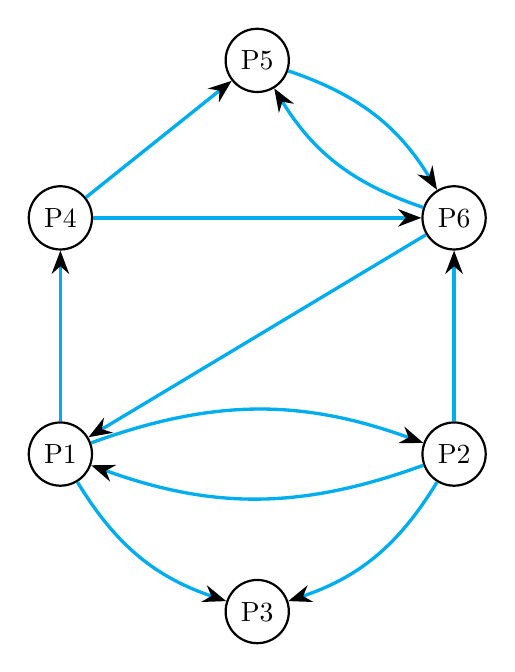
\begin{tikzpicture}
\begin{scope}[every node/.style={circle,thick,draw}]
	\node (P1) at (0,3) {P1};
	\node (P3) at (2.5,1) {P3};
	\node (P2) at (5,3) {P2} ;
	\node (P4) at (0,6) {P4};
	\node (P5) at (2.5,8) {P5};
	\node (P6) at (5,6) {P6} ;
\end{scope}			
\begin{scope}[>={Stealth[black]},
every node/.style={fill=white,circle},
every edge/.style={draw=cyan,very thick}]
\path [->] (P1) edge[bend left=20] (P2);
\path [->] (P1) edge[bend left=-20] (P3);
\path [->] (P1) edge[bend left=0] (P4);
\path [->] (P2) edge[bend left=20] (P1);
\path [->] (P2) edge[bend left=20] (P3);
\path [->] (P2) edge[bend left=0] (P6);
\path [->] (P4) edge[bend left=0] (P6);
\path [->] (P4) edge[bend left=0] (P5);
\path [->] (P5) edge[bend left=20] (P6);
\path [->] (P6) edge[bend left=0] (P1);
\path [->] (P6) edge[bend left=20] (P5);
\end{scope}
\end{tikzpicture}
\end{center}

A page is important if it is pointed to by other important pages.

\noindent Let's define PageRank of a page $P_{i}$, denoted $r\left(P_{i}\right)$ and it is the sum of the PageRanks of all pages pointing into $P_{i}$.
	
$$
r\left(P_{i}\right)=\sum_{P_{j} \in B_{P_{i}}} r\left(P_{j}\right)
$$
$B_{P_{i}}:$ is the set of pages pointing into $P_{i}$ \\
\\
The problem with formula is that the $r(P_{j})$ values, the PageRanks of pages inlinking to page $P_{i}$, are unknown. To sidestep this problem, we are going to use an iterative approach(process). That is, we are assuming that, in the beginning, all pages have equal PageRank (say, $1/n$, here $n$ is the number of web pages). As we are applying the rule in formula successively, we need to introduce some more notation in order to distinguish steps. Let $r_{k}\left(P_{i}\right)$ be the PageRank of page $P_{i}$ at $k^{th}$iteration. Then, PageRank of $P_i$ at $(k+1)^th$ iteration is given by
	
$$
r_{k+1}\left(P_{i}\right)=\sum_{P_{j} \in B_{P_{i}}} r_{k}\left(P_{j}\right)
$$
\begin{center}
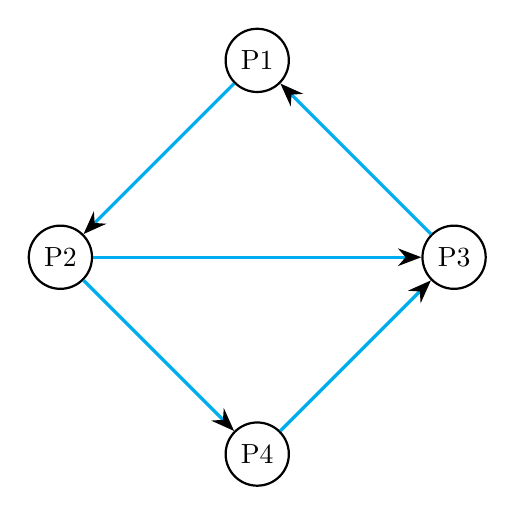
\begin{tikzpicture}
\begin{scope}[every node/.style={circle,thick,draw}]
\node (P4) at (2.5,3) {P4};
\node (P2) at (0,5.5) {P2};
\node (P1) at (2.5,8) {P1};
\node (P3) at (5,5.5) {P3} ;
\end{scope}
			
\begin{scope}[>={Stealth[black]},
every node/.style={fill=white,circle},
every edge/.style={draw=cyan,very thick}]
\path [->] (P1) edge[bend left=0] (P2);
				\path [->] (P2) edge[bend left=0] (P4);
				\path [->] (P2) edge[bend left=0] (P3);
				\path [->] (P4) edge[bend left=0] (P3);
				\path [->] (P3) edge[bend left=0] (P1);
			\end{scope}
		\end{tikzpicture}
	\end{center}
	
\noindent This process is initiated with $r_{0}\left(P_{i}\right)=1 / n$ for all pages $P_{i}$ and repeated with the hope that the PageRank scores will eventually converge to some final stable values. Applying equation to the above tiny web of 4-nodes gives the following values for the PageRanks after a few iterations.
\\

\begin{table}[h]
	\centering
	\begin{tabular}{l l l c}
		\toprule
		\textbf{Iteration 0} & \textbf{Iteration 1} & \textbf{Iteration 2} & \textbf{Iteration 3}\\
		\midrule
		$r_{0}\left(P_{1}\right)=1 / 4$ & $r_{1}\left(P_{1}\right)=1 / 4$ & $r_{2}\left(P_{1}\right)=2 / 4$ & 
		$r_{3}\left(P_{1}\right)=2 / 4$\\
		$r_{0}\left(P_{2}\right)=1 / 4$ & $r_{1}\left(P_{2}\right)=1 / 4$ & $r_{2}\left(P_{2}\right)=1 / 4$ & 
		$r_{3}\left(P_{2}\right)=2 / 4$\\
		$r_{0}\left(P_{3}\right)=1 / 4$ & $r_{1}\left(P_{3}\right)=2 / 4$ & $r_{2}\left(P_{3}\right)=2 / 4$ & 
		$r_{3}\left(P_{3}\right)=3 / 4$\\
		$r_{0}\left(P_{4}\right)=1 / 4$ & $r_{1}\left(P_{4}\right)=1 / 4$ & $r_{2}\left(P_{4}\right)=1 / 4$& 
		$r_{3}\left(P_{4}\right)=1 / 4$\\
		\bottomrule
	\end{tabular}
\end{table}

\noindent From the above table we can say that Page $P_3$ has highest rank and Page $P_4$ has lowest rank.\\
\\
\noindent This algorithm can be exploited by SEO's (Search Engine Optimization) by just creating dummy websites and pointing(more formally by giving backlinks) to their clients.\\
\\
\noindent This problem can be overcome by little change in previous algorithm.

$$
r\left(P_{i}\right)=\sum_{P_{j} \in B_{P_{i}}} \frac{r\left(P_{j}\right)}{\left|P_{j}\right|}
$$
$B_{P_{i}}:$ is the set of pages pointing into $P_{i}$ \\
$|P_{j}|:$ is the number of outlinks from page $P_{j}$.\\
\\
Recursive formula:
$$
r_{k+1}\left(P_{i}\right)=\sum_{P_{j} \in B_{P_{i}}} \frac{r_{k}\left(P_{j}\right)}{\left|P_{j}\right|} .
$$

\noindent Now, unlike previous algorithm dummy websites have no use as their value of backlinks decreases as the number of backlinks increase.

\begin{center}
	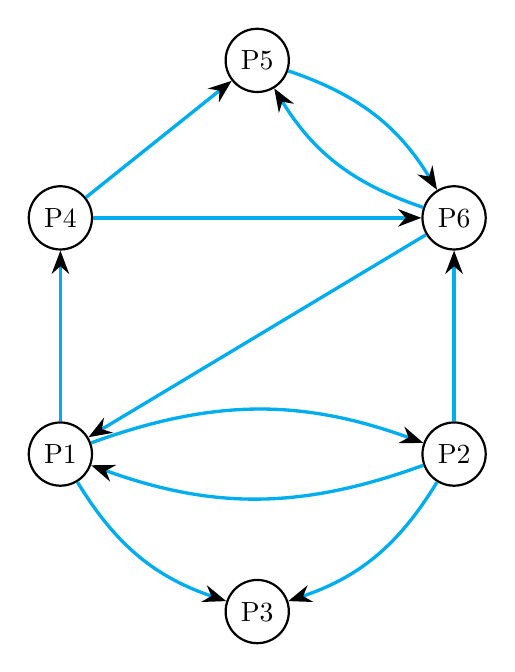
\begin{tikzpicture}
		\begin{scope}[every node/.style={circle,thick,draw}]
			\node (P1) at (0,3) {P1};
			\node (P3) at (2.5,1) {P3};
			\node (P2) at (5,3) {P2} ;
			\node (P4) at (0,6) {P4};
			\node (P5) at (2.5,8) {P5};
			\node (P6) at (5,6) {P6} ;
		\end{scope}
		\begin{scope}[>={Stealth[black]},
			every node/.style={fill=white,circle},
			every edge/.style={draw=cyan,very thick}]
			\path [->] (P1) edge[bend left=20] (P2);
			\path [->] (P1) edge[bend left=-20] (P3);
			\path [->] (P1) edge[bend left=0] (P4);
			\path [->] (P2) edge[bend left=20] (P1);
			\path [->] (P2) edge[bend left=20] (P3);
			\path [->] (P2) edge[bend left=0] (P6);
			\path [->] (P4) edge[bend left=0] (P6);
			\path [->] (P4) edge[bend left=0] (P5);
			\path [->] (P5) edge[bend left=20] (P6);
			\path [->] (P6) edge[bend left=0] (P1);
			\path [->] (P6) edge[bend left=20] (P5);
		\end{scope}
	\end{tikzpicture}
\end{center}
	
Let's calculate PageRank using updated algorithm,
	
\begin{table}[h]
	\centering
	\begin{tabular}{l l l c}
		\toprule
	\textbf{Iteration 0} & \textbf{Iteration 1} & \textbf{Iteration 2} & \textbf{PageRank}\\
		\midrule
		$r_{0}\left(P_{1}\right)=1 / 6$ & $r_{1}\left(P_{1}\right)=5 / 36$ & $r_{2}\left(P_{1}\right)=37 / 216$ & 3 \\
		$r_{0}\left(P_{2}\right)=1 / 6$ & $r_{1}\left(P_{2}\right)=2 / 36$ & $r_{2}\left(P_{2}\right)=10 / 216$ & 5 \\
		$r_{0}\left(P_{3}\right)=1 / 6$ & $r_{1}\left(P_{3}\right)=4 / 36$ & $r_{2}\left(P_{3}\right)=14 / 216$ & 4 \\
		$r_{0}\left(P_{4}\right)=1 / 6$ & $r_{1}\left(P_{4}\right)=2 / 36$ & $r_{2}\left(P_{4}\right)=10 / 216$ & 5 \\
		$r_{0}\left(P_{5}\right)=1 / 6$ & $r_{1}\left(P_{5}\right)=6 / 36$ & $r_{2}\left(P_{5}\right)=39 / 216$ & 2 \\
		$r_{0}\left(P_{6}\right)=1 / 6$ & $r_{1}\left(P_{6}\right)=11 / 36$ & $r_{2}\left(P_{6}\right)=46 / 216$ & 1\\			\bottomrule
		\end{tabular}
\end{table}
\end{document}